\section{Topological Entanglement Entropy}

\subsection{Topological Invariants}
A ``topological quantity'' is a quantity that is constant throughout every gapped phase. For example, if our quantity was $\Theta$, we could have the phase diagram like below, with $\Theta$ taking on a different value in each phase.

\begin{center}
    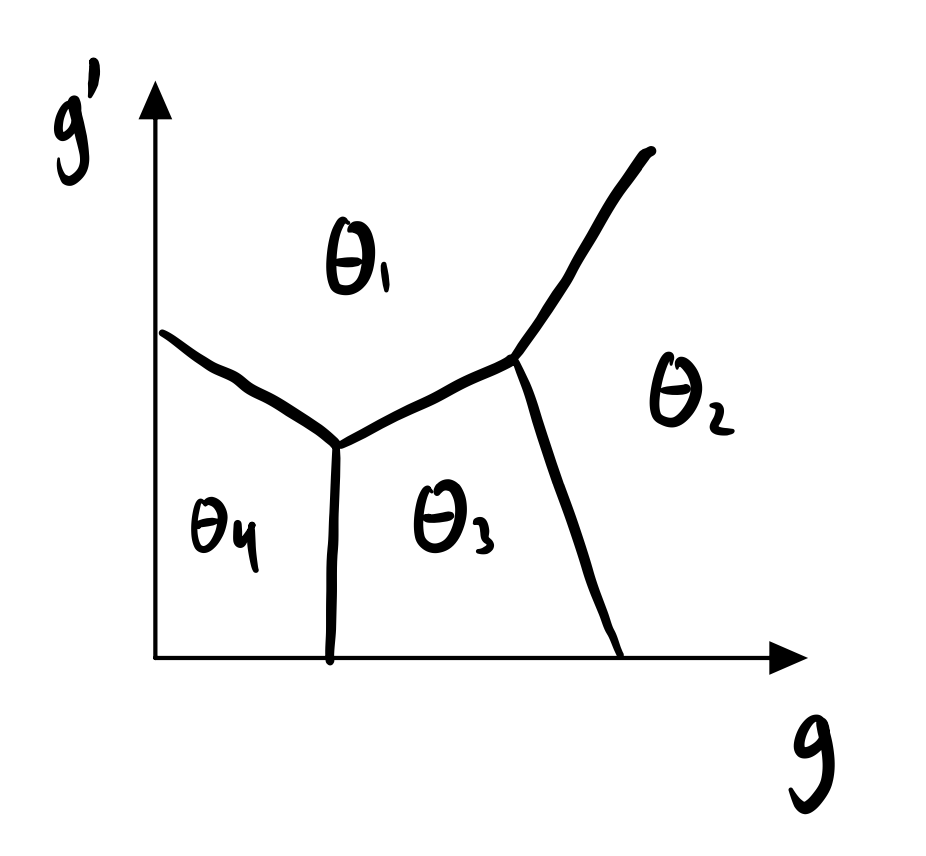
\includegraphics[scale=0.35]{Lectures/Images/lec17-phases.png}
\end{center}

Why ``topological''? In topology we say a quantity is topological if it is invariant to smooth deformations. Here, we can think that any path where the gap doesn't close (which is our analog of ``smoothness''), the topological quantity is invariant.

We expect that all topological quantities are completely determined by the ground state. An argument for this - we could have a scenario where we specified a state $\ket{\Omega}$, where person 1, 2 have different parent Hamiltonians $H, H'$ and calculate two different topological invariants. But, we know that this can't be the case; if we have two Hamiltonians with the same ground state, they belong to the same phase (we showed this on the homework), and hence must take the same value for $H, H'$. Thus, topological quantities only depend on $\ket{\Omega}$.

An important example is anyon data; e.g. the statistics of anyons and the number of anyon types. We expect that all of this anyon data must be encoded in the ground state. Today, we will think about how we will be able to extract this information. There are some recipes for this, but the only explicit formula comes from the topological entanglement entropy.

\subsection{Defining the Topological Entanglement Entropy}
We follow the discussion from (Levin \& Wen, \texttt{cond-mat/0510613}). 

Let $\ket{\Omega}$ be a gapped ground state on an infinite 2D lattice, and let $\rho = \dyad{\Omega}{\Omega}$. Consider an annulus, and split it up into the three regions:

\begin{center}
    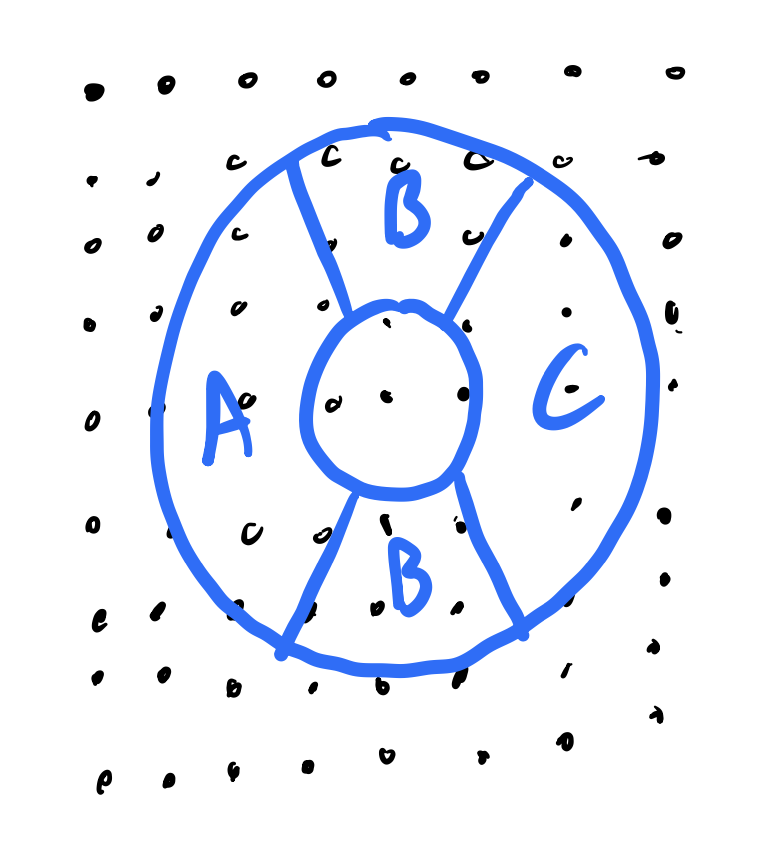
\includegraphics[scale=0.35]{Lectures/Images/lec17-TEE.png}
\end{center}

And define:
\begin{equation}
    \gamma = \frac{1}{2}\left[S(\rho_{AB}) + S(\rho_{BC}) - S(\rho_B) - S(\rho_{ABC})\right]
\end{equation}
in the limit of large $A, B, C$. We use $AB = A \cup B$, $BC = B \cup C$, and $ABC = A \cup B \cup C$. Equivalently, we can write:
\begin{equation}
    \gamma = \frac{1}{2}I(A:C\vert B)_\rho
\end{equation}
which is the ``quantum conditional mutual information''. 

Why are we interested in $\gamma$? It measures ``global'' correlations in ABC, in the sense that it measures correlations we would not have seen if we measured $AB, BC$ separately. This connect to anyons in that anyon excitations always have anyon string operators, which then give rise to global correlations.

Consider closed/open anyon string operators on the annulus:

\begin{center}
    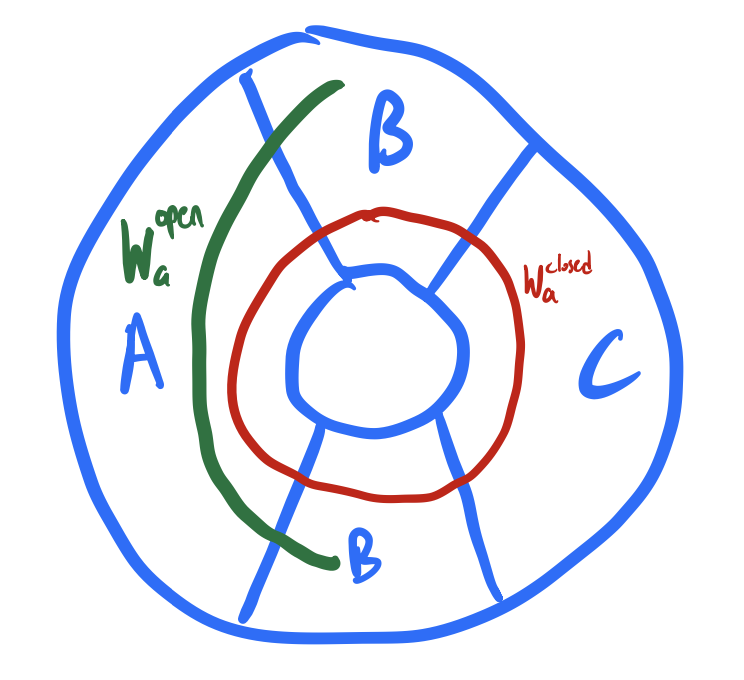
\includegraphics[scale=0.35]{Lectures/Images/lec17-stringops.png}
\end{center}

We then have that $\avg{W_a^{\text{closed}}} \neq 0$, but $\avg{W_a^{\text{open}}} = 0$ (as an open string creates two anyons at the end). Thus we expect that $\gamma > 0$ if $\ket{\Omega}$ supports nontrivial anyon excitations. Thus, we expect $\gamma > 0$ if $\ket{\Omega}$ supports nontrivial anyon excitations, $\gamma = 0$ otherwise.

\subsection{Alternative Definition of TEE}
This heuristic definition appears in (Kitaev/Preskill \texttt{hep-th/0510092}). Let $A$ be a disklike region.

\begin{center}
    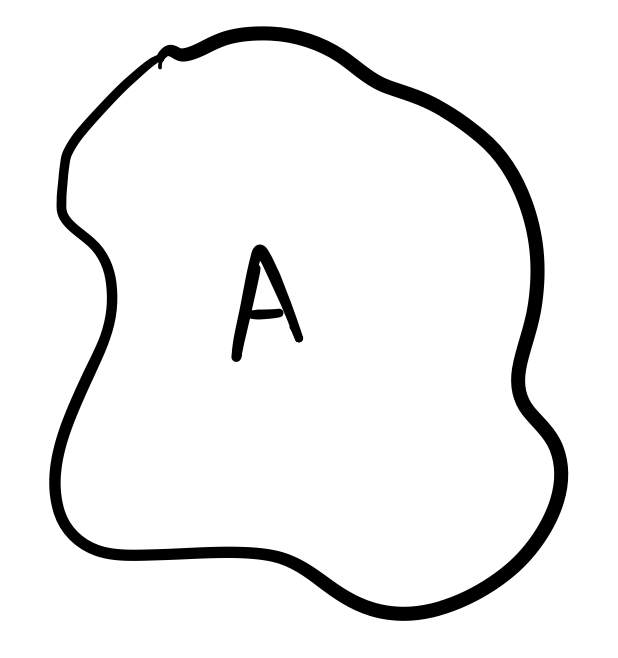
\includegraphics[scale=0.35]{Lectures/Images/lec17-regionA.png}
\end{center}
We then define the TEE $\gamma$ as a subleading correction to the area law:

\begin{equation}
    S(\rho_A) = \alpha\abs{\p A} - \gamma + \ldots
\end{equation}
Note that the area law is $O(L)$ and the TEE is the $O(1)$ constant correction.

This is difficult to make sense of on a lattice, where $\abs{\p A}$ is not so well defined (sometimes people consider an embedding onto a cylinder to make the notion of the perimeter precise).

This formula gives a nice alternative perspective on our first definition for $\gamma$, where we can see that all of the area law terms cancel out and leave just $\gamma$.

\subsection{Original conjecture for anyons}
the original conjecture was that for any gapped state $\ket{\Omega}$:
\begin{equation}
    \gamma = \log \mathcal{D}
\end{equation}
where $\mathcal{D} = \sqrt{\sum_a d_a^2}$ is the total quantum dimension, where $d_a$ is the quantum dimension of anyon $a$. The sum is over all anyon types, including the trivial anyon.

The ``quantum dimension'' of an anyon $a$ is defined by:
\begin{equation}
    d_a = \lim_{n\to\infty}\left(\text{topological degeneracy of $n$ $a$'s}\right)^{1/n}
\end{equation}

Some examples; for Abelian anyons $a$, we have $d_a = 1$ (and the converse is also true). For non-Abelian anyons, we have that $d_a > 1$ (again this is an iff statement). The quantum double model the quantum dimension is the size of the conjugacy classes. 

An important special case; if $\ket{\Omega}$ supports only Abelian anyon excitations, then $\mathcal{D} = \sqrt{\text{\# of anyon types}}$ as $d_a = 1$ for each type.

If we are in the trivial phase, we have $\mathcal{D} = 1$ and so the prediction is $\gamma = \log \mathcal{D} = 0$. For the toric code, we have anyon types $\set{1, e, m, \e}$, so then $\mathcal{D} = 2$ and so the prediction is $\gamma = \log \mathcal{D} = \log 2$.

\subsection{Status of the conjecture}
This conjecture has been verified for many many examples.
\begin{itemize}
    \item Exactly solvable models
    \item Many numerical (unsolvable) examples
    \item Supported by field theory arguments
\end{itemize}
The general belief is thus that it works generically. However - finely tuned counterexamples have been found.

Bravyi's counterexample is a simple 1D state, but drawn in 2D.

\begin{center}
    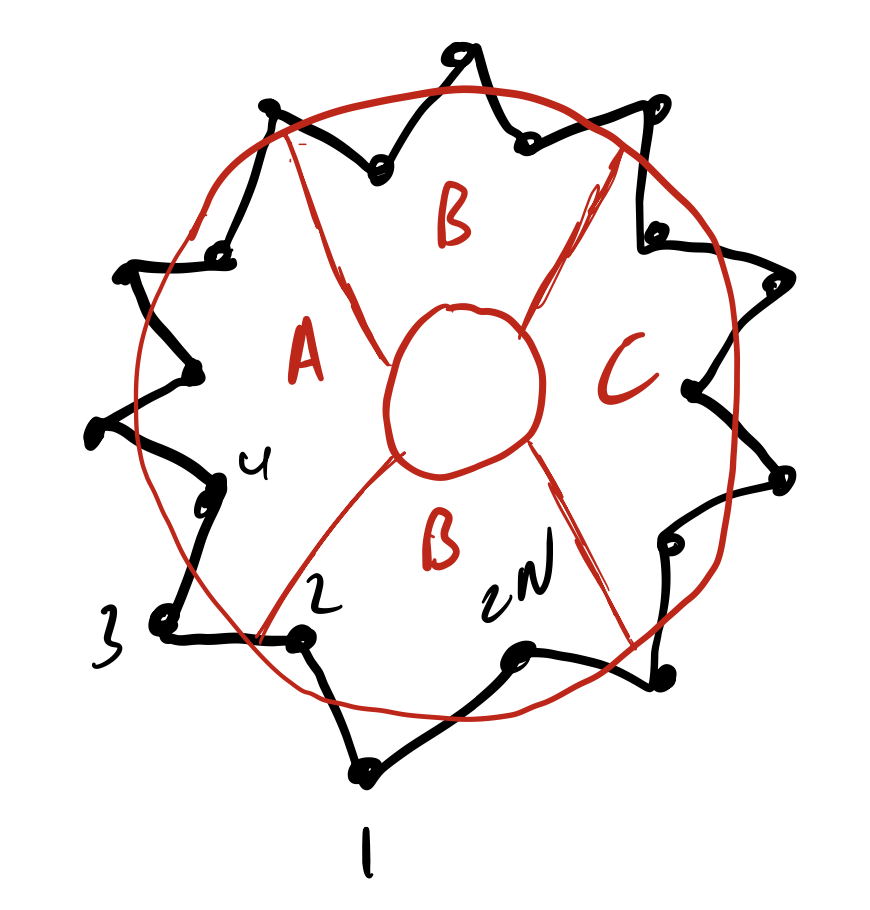
\includegraphics[scale=0.35]{Lectures/Images/lec17-TEEcounterexample.png}
\end{center}

Consider the ground state of:
\begin{equation}
    H = -\sum_{i=1}^{2N}Z_{i-1}X_iZ_{i+1}
\end{equation}
which is the cluster state $\ket{\Psi_{CS}}$. This is a short-range entangled state (it can be prepared from a product state via a finite (constant) depth circuit), so there are definitely no anyons. So if we were to believe the conjecture, we should get $\gamma = 0$. But, if we calculate this, we find:
\begin{equation}
    \gamma = \frac{1}{2}\log 2 > 0
\end{equation}
independent of $N$, which is a counterexample.

Two comments; you could object that this is not a 2D state. But, we could consider just embedding this into a 2D lattice where the other sites were just unentangled product state. Then you might argue that the lattice is not translationally invariant, and we are constructing a series of states. But to that we can say that there are truly 2D examples with a similar flavour; this is just the simplest one.

Why do we get $\gamma > 0$? Notice that:
\begin{equation}
    X_2X_4\ldots X_{2N}\ket{\Psi_{CS}} = \ket{\Psi_{CS}}
\end{equation}
which is a truly global correlation on ABC; compare this to the fact that:
\begin{equation}
    \avg{X_2X_4\ldots X_{2k}} = 0
\end{equation}
for $k < N$ (as this anticommutes with one term in the Hamiltonian).

We say that $\ket{\Psi_{CS}}$ has a ``spurious TEE''; it comes from spurious global correlation that has nothing to do with anyons. We might then ask what is the precise universal relationship between the TEE and the anyon data. It turns out to be that there is a universal inequality relating the two:
\begin{equation}
    \boxed{\gamma \geq \log \mathcal{D}}
\end{equation}
which can be proved rigorously for all gapped states. It tells us that $\gamma$ doesn't tell us about the number of anyons precisely, but it gives an upper bound to the anyon content. This is natural - our intuitive argument was that anyons give global correlations that add to $\gamma$. But the converse direction was hard to argue - why isn't there global correlations coming from other sources? Indeed, the new formula captures the fact that you could have extra correlations (e.g.z the spurious global correlations in the cluster state example). The inequality (which we note applies to the first definition we gave) is thought to be saturated for ``generic'' states.

Some examples of using $\gamma$ in practice:
\begin{enumerate}
    \item If $\gamma = 0$, then we are certain $\mathcal{D} = 1$ and so we have no nontrivial anyons.
    \item If $\gamma = \frac{1}{2}\log 2$ then $\mathcal{D} \leq \sqrt{2}$; then we have at most one nontrivial anyon.
\end{enumerate}